\documentclass[border=15pt, multi, tikz]{standalone}
\usepackage{import}
\subimport{./layers/}{init}
\usetikzlibrary{positioning}
\usetikzlibrary{3d} % input image

\def\ConvColor{rgb:yellow,5;red,2.5;white,5}
\def\ConvReluColor{rgb:yellow,5;red,5;white,5}
\def\PoolColor{rgb:red,1;black,0.3}
\def\FcColor{rgb:blue,5;red,2.5;white,5}
\def\FcReluColor{rgb:blue,5;red,5;white,4}

\begin{document}
\begin{tikzpicture}

% Box.sty and RightBandedBox.sty were modified:
% \tikzstyle{depthlabel}=[pos=0.5,text width=14*\z,text centered,sloped] % pos=0 was the default
% \tikzstyle{captionlabel}=[text width=15*\LastEastx/\scale,text centered,anchor=north,text height=0,inner sep=0,outer sep=0] % anchor=north,text height=0,inner sep=0,outer sep=0 was added

\tikzstyle{connection}=[ultra thick,every node/.style={sloped,allow upside down},draw=\edgecolor,opacity=0.7]

%%%%%%%%%%%%%%%%%%%%%%%%%%%%%%%%%%%%%%%%%%%%%%%%%%%%%%%%%%%%%%%%%%%%%%%%%%%%%%%%%%%%%%%%
%% Draw Layer Blocks
%%%%%%%%%%%%%%%%%%%%%%%%%%%%%%%%%%%%%%%%%%%%%%%%%%%%%%%%%%%%%%%%%%%%%%%%%%%%%%%%%%%%%%%%
% image
\node[canvas is zy plane at x=0] (temp) at (-3,0,0) {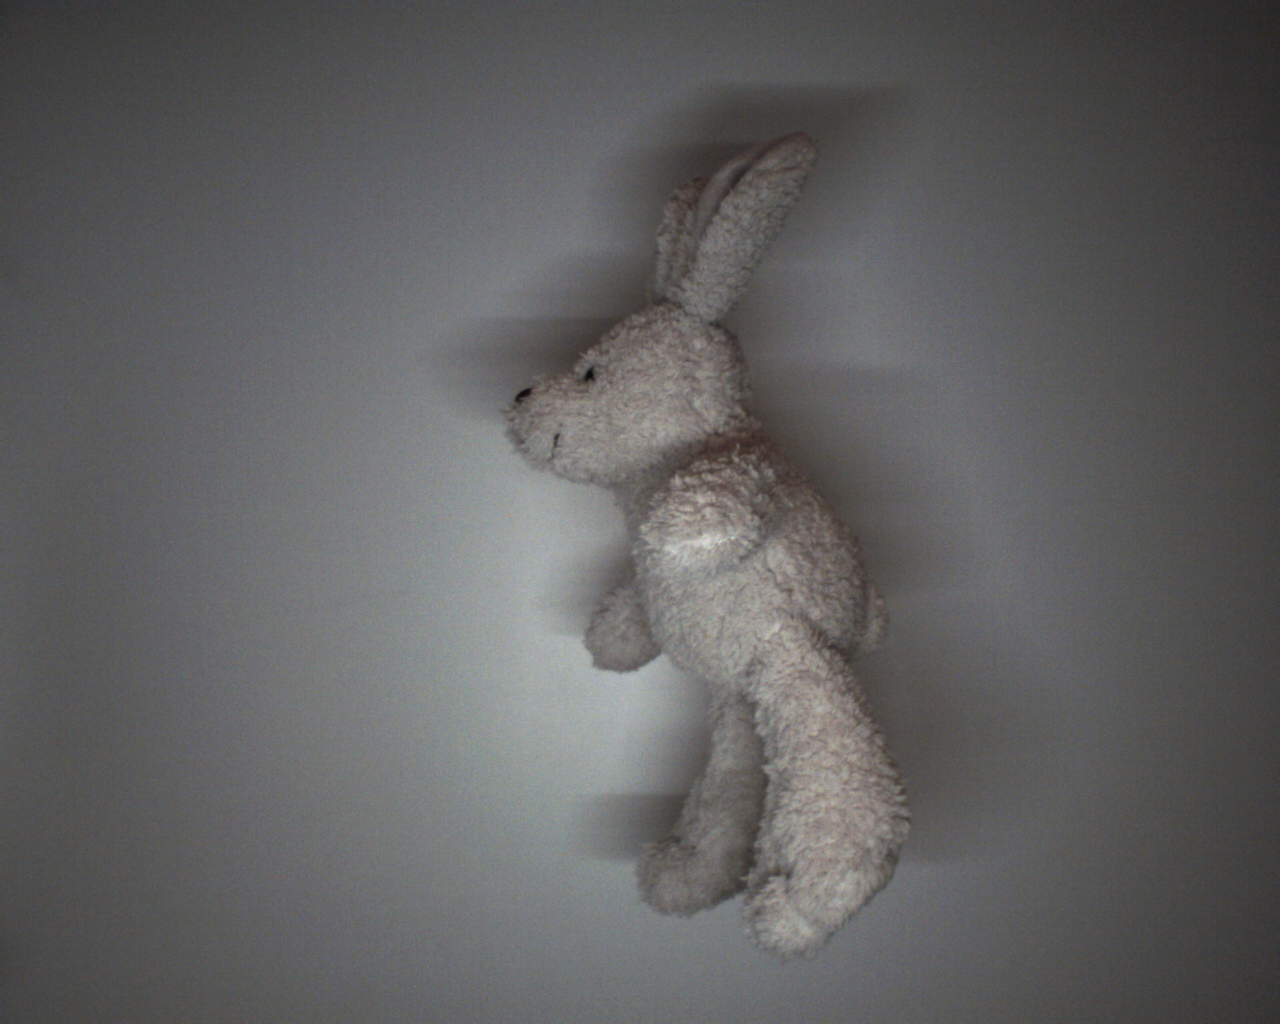
\includegraphics[width=15.059072cm,height=12.0472576cm]{1574952009_278_10_stuffed-bunny.png}};
%%%%%%%%%%
% conv1
\pic[shift={(0,0,0)}] at (0,0,0) {RightBandedBox={name=cr1,caption=conv1\\5~$\times$~5\\pool1\\2~$\times$~2,%
        xlabel={{"16",""}},ylabel=256,zlabel=320,fill=\ConvColor,bandfill=\ConvReluColor,%
        height=60.236288,width={2},depth=75.29536}};
% pool1
\pic[shift={(0,0,0)}] at (cr1-east) {Box={name=p1,%
        fill=\PoolColor,opacity=0.5,height=43.02592,width=1,depth=53.7824}};
%%%%%%%%%%
% conv2
\pic[shift={(2.3,0,0)}] at (p1-east) {RightBandedBox={name=cr2,caption=conv2\\3~$\times$~3\\pool2\\2~$\times$~2,%
        xlabel={{"32",""}},ylabel=128,zlabel=160,fill=\ConvColor,bandfill=\ConvReluColor,%
        height=43.02592,width={4},depth=53.7824}};
% pool2
\pic[shift={(0,0,0)}] at (cr2-east) {Box={name=p2,%
        fill=\PoolColor,opacity=0.5,height=30.7328,width=1,depth=38.416}};
%%%%%%%%%%
% conv3
\pic[shift={(2,0,0)}] at (p2-east) {RightBandedBox={name=cr3,caption=conv3\\3~$\times$~3\\pool3\\2~$\times$~2,%
        xlabel={{"32",""}},ylabel=64,zlabel=80,fill=\ConvColor,bandfill=\ConvReluColor,%
        height=30.7328,width={4},depth=38.416}};
% pool3
\pic[shift={(0,0,0)}] at (cr3-east) {Box={name=p3,%
        fill=\PoolColor,opacity=0.5,height=21.952,width=1,depth=27.44}};
%%%%%%%%%%
% conv4
\pic[shift={(1.7,0,0)}] at (p3-east) {RightBandedBox={name=cr4,caption=conv4\\3~$\times$~3\\pool4\\2~$\times$~2,%
        xlabel={{"64",""}},ylabel=32,zlabel=40,fill=\ConvColor,bandfill=\ConvReluColor,%
        height=21.952,width={8},depth=27.44}};
% pool4
\pic[shift={(0,0,0)}] at (cr4-east) {Box={name=p4,%
        fill=\PoolColor,opacity=0.5,height=15.68,width=1,depth=19.6}};
%%%%%%%%%%
% conv5
\pic[shift={(1.4,0,0)}] at (p4-east) {RightBandedBox={name=cr5,caption=conv5\\3~$\times$~3\\pool5\\2~$\times$~2,%
        xlabel={{"64",""}},ylabel=16,zlabel=20,fill=\ConvColor,bandfill=\ConvReluColor,%
        height=15.68,width={8},depth=19.6}};
% pool5
\pic[shift={(0,0,0)}] at (cr5-east) {Box={name=p5,%
        fill=\PoolColor,opacity=0.5,height=11.2,width=1,depth=14}};
%%%%%%%%%%
% conv6
\pic[shift={(1.1,0,0)}] at (p5-east) {RightBandedBox={name=cr6,caption=conv6\\3~$\times$~3\\pool6\\2~$\times$~2,%
        xlabel={{"128",""}},ylabel=8,zlabel=10,fill=\ConvColor,bandfill=\ConvReluColor,%
        height=11.2,width={16},depth=14}};
% pool6
\pic[shift={(0,0,0)}] at (cr6-east) {Box={name=p6,%
        fill=\PoolColor,opacity=0.5,height=8,width=1,depth=10}};
%%%%%%%%%%
% conv7
\pic[shift={(0.9,0,0)}] at (p6-east) {RightBandedBox={name=cr7,caption=conv7\\3~$\times$~3,%
        xlabel={{"128",""}},ylabel=4,zlabel=5,fill=\ConvColor,bandfill=\ConvReluColor,%
        height=8,width={16},depth=10}};
%%%%%%%%%%
% fc8
\pic[shift={(3,0,0)}] at (cr7-east) {RightBandedBox={name=fc8,caption=fc8,%
        xlabel={{"1",""}},ylabel=1,zlabel=512,fill=\FcColor,bandfill=\FcReluColor,%
        height=3,width=3,depth=100}};
%%%%%%%%%%
% fc9
\pic[shift={(2,0,0)}] at (fc8-east) {Box={name=fc9,caption=fc9,%
        xlabel={{"1",""}},ylabel=1,zlabel=22,fill=\FcColor,%
        height=3,width=3,depth=25}};

%%%%%%%%%%%%%%%%%%%%%%%%%%%%%%%%%%%%%%%%%%%%%%%%%%%%%%%%%%%%%%%%%%%%%%%%%%%%%%%%%%%%%%%%
%% Draw Arrow Connections
%%%%%%%%%%%%%%%%%%%%%%%%%%%%%%%%%%%%%%%%%%%%%%%%%%%%%%%%%%%%%%%%%%%%%%%%%%%%%%%%%%%%%%%%
\draw [connection]  (p1-east)        -- node {\midarrow} (cr2-west);
\draw [connection]  (p2-east)        -- node {\midarrow} (cr3-west);
\draw [connection]  (p3-east)        -- node {\midarrow} (cr4-west);
\draw [connection]  (p4-east)        -- node {\midarrow} (cr5-west);
\draw [connection]  (p5-east)        -- node {\midarrow} (cr6-west);
\draw [connection]  (p6-east)        -- node {\midarrow} (cr7-west);
\draw [connection]  (cr7-east)        -- node {\midarrow} (fc8-west);
\draw [connection]  (fc8-east)       -- node {\midarrow} (fc9-west);
% \draw [connection]  (fc9-east)       -- node {\midarrow} ++(1.5,0,0);

%%%%%%%%%%%%%%%%%%%%%%%%%%%%%%%%%%%%%%%%%%%%%%%%%%%%%%%%%%%%%%%%%%%%%%%%%%%%%%%%%%%%%%%%
%% Draw Dotted Edges 
%%%%%%%%%%%%%%%%%%%%%%%%%%%%%%%%%%%%%%%%%%%%%%%%%%%%%%%%%%%%%%%%%%%%%%%%%%%%%%%%%%%%%%%%
\draw[densely dashed]
    (fc8-west)++(0, 1.5*.2, 1.5*.2) coordinate(a) -- (cr7-nearnortheast)
    (fc8-west)++(0,-1.5*.2, 1.5*.2) coordinate(b) -- (cr7-nearsoutheast)
    (fc8-west)++(0,-1.5*.2,-1.5*.2) coordinate(c) -- (cr7-farsoutheast)
    (fc8-west)++(0, 1.5*.2,-1.5*.2) coordinate(d) -- (cr7-farnortheast)
    
    (a)--(b)--(c)--(d)
    ;

\end{tikzpicture}
\end{document}
